\documentclass[10pt]{article}
\usepackage[a4paper, left=2.5cm, right=2.5cm, top=2.5cm, bottom=2cm]{geometry}
%font managment
\usepackage[T1]{fontenc}
\usepackage{fontspec}
%\setmainfont[SizeFeatures={Size=10}]{Roboto Condensed}
\setmainfont[SizeFeatures={Size=10}]{Source Sans Pro}
\usepackage{xcolor}

\usepackage{setspace}
\usepackage{float}
\usepackage{pdfpages}
\usepackage{graphicx}
\usepackage{wrapfig}
%bibliography
%\usepackage[nottoc,notlof,notlot]{tocbibind} 
\usepackage[nottoc,numbib]{tocbibind}
\usepackage[backend=biber]{biblatex}
\renewcommand*{\bibfont}{\fontspec{Source Sans Pro}}
\addbibresource{quotes/DBLiteratur.bib}
\addbibresource{quotes/rust.bib}
\addbibresource{quotes/RPI.bib}
\usepackage[ngerman]{babel}
\usepackage{csquotes}
%einfuegen eines Logos
%set URL font to default
\urlstyle{same}

%for wrapfigure:

\usepackage{longtable}

\usepackage{svg}

\usepackage[formats]{listings}


\usepackage{subcaption}
\DeclareFieldFormat{urldate}{, aufgerufen am #1}

\usepackage{hyperref}
\hypersetup{
    colorlinks,
    citecolor=black,
    filecolor=black,
    linkcolor=black,
    urlcolor=black
}

\begin{document}
\begin{titlepage}
\vspace*{\stretch{1}}
\begin{center}
%\textsc{\Large %Jugend Forscht Arbeit 2023}\\ 
%\includesvg[width=0.15\textwidth]{Jugend_forscht.svg}\centering Arbeit 2023}
{
\hspace{1.5em}
\begin{minipage}[c]{0.15\textwidth}
\vspace{0.15em}
\includesvg[width=\textwidth]{Jugend_forscht.svg}
\end{minipage}
\begin{minipage}[c]{0.15\textwidth}
 {\huge Arbeit 2023}
\end{minipage}
}
%}
\\[9ex]
{\centerline{\huge\bfseries helper:Paper} 
\large \bfseries Entwicklung und Einsatz von ressourcenschonenden\\
Smart Clocks am Beispiel von Schulen}
 
\vspace{6ex}
\centerline{

\includegraphics[width=0.3\textwidth]{helperPaper_Logo.jpg}
}
\vspace{20ex}
{\large\bfseries  Linda Gemeinhardt - Ben Mattes Krusekamp} \\
\vspace{2ex}
\centerline{\large Unter der Betreuung von Hendrik Büdding}
\vspace{6ex}
\vfill
%\vfill
\includesvg[width=0.15\textwidth]{annette-logo.svg} \\
\vspace{1ex}
\large Annette-von-Droste-Hülshoff-Gymnasium Münster  \\
%Grüne Gasse 38, 48143 Münster                                 
  \vfill
  \today
\end{center}
\vspace{\stretch{2}}

%\newpage
%\thispagestyle{empty}
%{\centerline{\huge\bfseries Kurzfassung}}
%\vspace{6ex}
%Das helper:Paper ist eine vielseitig einsatzbare Alltagsunterstützung, die alle wichtigen Informationen für einen strukturierten Tag beinhaltet. So können individuelle Widgets (wie zum Beispiel ein Uhr-, Kalender- oder Wetterwidget) per App ausgewählt und auf diesem projiziert werden.

%Das helper:Paper umfasst als Anzeige ein stromsparendes E-Paper - insofern wird Digitales mit Nachhaltigkeit verbunden.

%In dieser Projektarbeit wurde das helper:Paper auf den Anwendungsbereich Schule angepasst. Andere denkbare Anwendungsbereiche wären das häusliche Umfeld oder der Einsatz in Unternehmen. Die Schule bietet Raum zur Verbesserung der Digitalisierung und der technischen Infrastruktur. Das helper:Paper soll dabei den Schulalltag der Schüler*Innen und Lehrer*Innen vereinfachen (Zeitmanagement).

%In Schulen soll das helper:Paper unter anderen die Türschilder, Uhranzeigen und die Vertretungs- und Belegungspläne ersetzen und auf Augenhöhe neben den Klassen- und Fachräumen angebracht werden.

\end{titlepage}
\thispagestyle{empty}
\setcounter{secnumdepth}{3}
\setcounter{tocdepth}{3}
\pagenumbering{gobble}
\renewcommand*\contentsname{Inhaltsverzeichnis}
\tableofcontents
\clearpage
\pagenumbering{roman}
\setcounter{page}{1}
%Kurzfassung mit Foto (Arbeit/helper:Paper anpreisen)
\setcounter{secnumdepth}{-1}
\section{Kurzfassung}
Das helper:Paper ist eine vielseitig einsetzbare Alltagsunterstützung, die alle wichtigen Informationen für einen strukturierten Tag beinhaltet. So können individuelle Widgets (wie zum Beispiel ein Uhr-, Kalender-, Wetter-, Busplan-, Belegungsplan- und/oder Notizfeld-Widget) per App ausgewählt und auf das helper:Paper projiziert werden.

Das helper:Paper umfasst als Anzeige ein E-Paper-Display und ist dadurch stromsparend – insofern wird Digitales mit Nachhaltigkeit verbunden.

In dieser Projektarbeit wird das helper:Paper auf den Anwendungsbereich Schule angepasst. Andere denkbare Anwendungsbereiche mit Potenzial sind Behörden, öffentliche Einrichtungen, das häusliche Umfeld sowie der Einsatz in Unternehmen.
Die Schule bietet viel Raum zur Verbesserung der Digitalisierung und der technischen Infrastruktur. Das helper:Paper soll das aufgreifen und den Schulalltag der Schüler*innen, Lehrer*innen und der Verwaltungs- und Fachkräfte vereinfachen.

In Schulen soll das helper:Paper unter anderen die Türschilder, Uhranzeigen und die Vertretungs- beziehungsweise Belegungspläne ersetzen und auf Augenhöhe neben den Klassen-, Kurs- und Fachräumen angebracht werden. Somit können wichtige Informationen (zum Beispiel die funkgenaue Zeit) im Vorbeigehen gelesen werden. Auch kurzfristige Raumänderungen sollen eingeblendet werden. Das Zeitmanagement der Schüler*innen und Lehrer*innen soll so insgesamt positiv verbessert werden und weniger Unterrichtsstörungen stattfinden. 
\setcounter{secnumdepth}{3}

\begin{figure}[h]
  \centerline{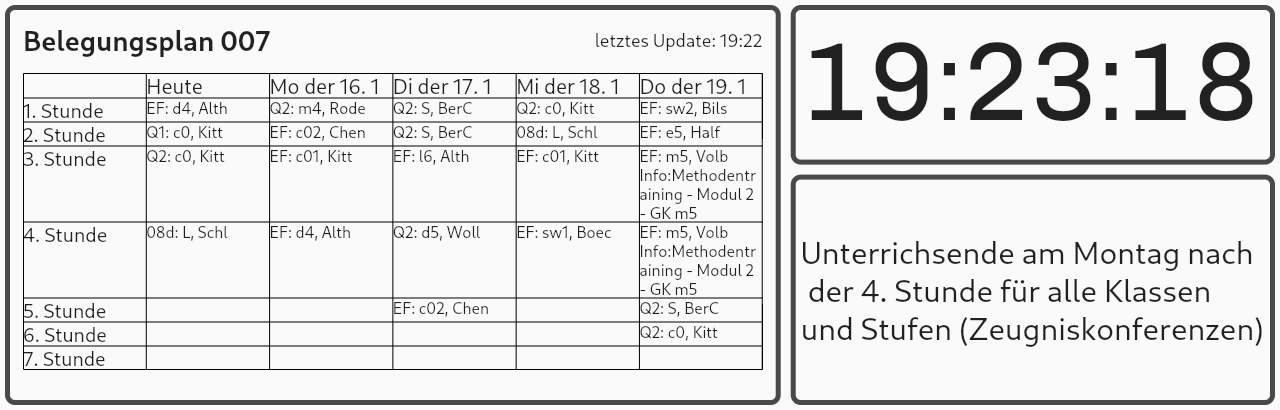
\includegraphics[width=0.9\textwidth]{Screenshot_20230113_192318.png}}
  \caption{helper:Paper Anzeige}
  \label{Vorderseite helper:Paper}
\end{figure}

Die Schüler*innen aller Jahrgangsstufen hätten somit zu jeder Zeit direkten Zugang zu den aktuellen und individuellen Vertretungsplänen. Sie müssten nicht mehr mehrmals am Tag zum zentralen Vertretungsplan gehen, um dort zu warten, bis die Rotation auf dem Monitor ihre Klasse anzeigt, sondern könnten vor ihrem Klassenraum den individuellen Plan für ihre Klasse sehen.

Die Lehrer*innen könnten auf dem helper:Paper erkennen, ob der Nachbarraum frei ist, um dort Gruppenarbeiten zu ermöglichen, ohne gegebenenfalls den Unterricht stören zu müssen. Sie könnten ebenso sehen, ob ein Fachraum (zum Beispiel ein Computerraum) kurzfristig frei ist. Dazu müssten sie nicht mehr zum Stundenplanbüro oder Sekretariat gehen, um dort nachzufragen. Verwaltungs- und Fachangestellte könnten somit mit weniger Unterbrechungen ihrer Arbeit nachgehen. Auch würden sie Wege und Zeit sparen, statt aktualisierte Türbeschilderungen auszutauschen. Das helper:Paper aktualisiert sich per Mausklick!
\clearpage
\pagenumbering{arabic}
\setcounter{page}{1}
\section{Einleitung} 
„Der Bund unterstützt Länder und Gemeinden bei Investitionen in die digitale kommunale Bildungsinfrastruktur. […] Sie verpflichten sich gemeinsam mit den Kommunen zur Sicherstellung von Betrieb und Wartung der technischen Infrastruktur“ \cite{Digitalisierung}. 
In Nordrhein-Westfalen fokussiert der Ausbau der Infrastruktur „schnelles Internet und neue Computer in Schulen“ \cite{Digitalisierung}.
Auch die Bundesregierung hat den Verbesserungspotential „Schule“ in Bezug auf Digitalität und technischen Infrastruktur erkannt und setzt sich für eine Verbesserung in Form von Investitionen ein. In dieser Arbeit werden neben der Digitalisierung ein Fokus auf die Nachhaltigkeit gelegt.

%Diese Arbeit ist im Rahmen des Projektkurses Informatik der Oberstufe entstanden, dessen Zielrichtung "digital und nachhaltig“ ist. 
Die Entwicklung und der Einsatz von ressourcenschonenden und zukunftsträchtigen Smart Clocks, dem helper:Paper, wird in der Projektarbeit thematisiert. Das helper:Paper wurde als Beispiel auf den Anwendungsort Schule angepasst. Möglich ist auch der Einsatz in öffentlichen Einrichtungen, in Unternehmen oder im häuslichen Umfeld.
%In der Praxis wurden exemplarisch einige Widgets für die weiteren Anwendungsbereiche erstellt. 
Des Weiteren werden die aufgestellten und angenommenen Thesen zur Umsetzung und Nutzung eines helper:Papers in Form einer Grundlagenstudie überprüft.

\subsection{Forschungsfrage}
Grundlage der Forschungsfrage ist das helper:Paper - die Idee sowie die Entwicklung und die Spezifizierung auf den Anwendungsbereich Schule. Die gesammelten Erfahrungen der Autorin und des Autors dieser Arbeit und das von ihnen erkannte Potenzial in der Schule stellen den Anfang des Projektes dar. Die Anwendung und Entwicklung des helper:Papers kann unter anderem auch auf öffentliche Gebäude ausgeweitet werden. Es soll den Alltag vereinfachen und seinen Teil zum Klimaschutz beitragen. 

Darauf basierend wurde untersucht, ob der Einsatz des helper:Papers dazu beitragen kann, den Stromverbrauch in Schulen zu senken und, ob dort die \glqq Arbeitsqualität" (die Organisation und die Informationsverbreitung) optimiert werden kann. \label{Verbesserung Arbeitsqualität?}

%keine Handys für Unterstufe
\subsection{Motivation}
Die zentrale Vertretungsplan-Anzeige in Schulen verbraucht im Gegensatz zu einem E-Paper relativ viel Strom (siehe \ref{Strommessung}). Auch sind die analogen Aushänge oder Belegungspläne der Fachräume oftmals nicht aktuell und befinden sich an den Türinnenseiten. 

Vor den Klassenräumen hängen Raumschilder mit Klassenstufen (wie zum Beispiel 5a, 9d), den jeweiligen Namen der Klassenlehrer*innen und in der Türinnenseite ein Stundenplan. Diese müssen bei jeder Änderung – spätestens zum neuen Schuljahr – erneuert werden. Dazu werden die Informationen quartalsweise auf Papier gedruckt und durch Personal am jeweiligen Raum angebracht.

Hinsichtlich des Klimawandels müssen dringend Wertstoffe (hier: Papier und Wasser) und Ressourcen (hier: Strom) eingespart werden \cite{Ressourcenschutz}.

Geräte, die viel Energie verbrauchen, müssen ersetzt werden. „Für den weltweiten Klimaschutz [trage] Deutschland als führende Industrienation eine besondere Verantwortung. Klimaschutz [gehe] jeden etwas an [und es sei] eine gemeinsame Kraftanstrengung“ \cite{Klimaschutzprogramm}.

%Für den Anwendungsort Schule lässt sich eine sekundäre Frage formulieren: Erhöht sich durch den Einsatz des helper:Papers die Arbeitseffektivität?

%Ressourcenschonenden Smart Clocks ,helper:Paper, können auch im häuslichen Umfeld sowie in Unternehmen oder anderen öffentlichen Gebäuden ihren Einsatz finden.

\subsection{Zielsetzung}
Im Rahmen dieser Arbeit wird das helper:Paper schematisch entwickelt, der Stromverbrauch untersucht, das Kosten-Nutzen-Verhältnis analysiert und eine empirische Studie (Grundlagenstudie) zur Eignung des helper:Papers erstellt werden. Der Fokus wird auf den Anwendungsbereich Schule gelegt. 

% verwendete Soft und Hardware aufbau und gestützt werden nicht neutral: 
%Ziel dieser Projektarbeit ist die Entwicklung des helper:Papers, als ersten Fokus spezialisiert auf den Anwendungsbereich Schule. Im Zuge der Entwicklung des helper:Papers wird die verwendete Soft- und Hardware erläutert. Die Zielsetzung soll unter anderem durch eine empirische Studie (Grundlagenstudie) zur Eignung des helper:Papers in Schulen gestützt werden.

\subsection{Aufbau der Arbeit}
Der Definition, der Motivation und der Entwicklung zur gestellten Forschungsfrage und deren Ziel folgen die Namensgebung und die Erläuterungen zum Vorgehen und zur eingesetzten Soft- und Hardware. Neben den unterschiedlichen Programmen zur Entwicklung des helper:Papers wird auf die Hardware für die Anzeige (E-Paper) und den Raspberry PI (Einplatinen-Computer) eingegangen. Die Funktionsweise und die Bedienung des helper:Papers sowie die Implementierung der grafischen Applikationen und des E-Papers werden aufgezeigt. Darauf folgt eine wissenschaftliche Erarbeitung in Form einer Analyse der Ausgangslage und eine Strommessung einer herkömmlichen Vertretungsplananzeige (Stromverbrauch im Vergleich und Stromkosten im Vergleich).
Die gesetzten Annahmen zum Einsatz des helper:Papers werden in einer empirischen Studie (Grundlagenstudie) mithilfe von 211 Probandinnen und Probanden überprüft, ausgewertet und evaluiert. In der abschließenden Diskussion zur Soft-, Hardware, Strommessung und der empirischen Studie werden Ergebnisse reflektiert, ein Fazit und Erweiterungsmöglichkeiten des helper:Papers sowie Potenziale für die Praxis aufgezeigt.

\subsection{Namensgebung}
Der Neologismus \textit{helper:Paper} setzt sich aus den Wörtern \textit{helper} (engl. für Helfer*in) und \textit{paper} (engl. für Papier) zusammen. Das \textit{paper} steht für das verwendete E-Paper und \textit{helper} beschreibt die Funktion des helper:Papers. Sie soll den Alltag vereinfachen und eine Hilfestellung sein. 

Die beiden Wörter wurden mithilfe eines Smileys (:P) verbunden, das auch im Logo aufgegriffen wurde. 

%Projektbeschreibung in Einleitung
%siehe Soft Hardwarekomponenten zwei
\section{Vorgehensweise, Methoden und Materialien}\label{Methoden-Material}
Um die Entwicklung des helper:Papers zu ermöglichen, werden drei Soft- und drei Hardwarekomponenten benötigt.

\paragraph{Verwendete Software}
Die drei benötigten Softwarekomponenten teilen sich in Ansteuerung des E-Papers, der Bildgenerierung für das E-Paper sowie eine Software, die die Konfiguration und Individualisierung des helper:Papers erlaubt, auf. Letzteres könnte auch durch bestehende Programme, wie \textit{SSH} \footnote{SSH ist ein Programm, um auf die Befehlszeile eines externen Rechners zuzugreifen.}, erfüllt werden. Diese Lösung wurde nicht favorisiert, 
da davon ausgegangen wurde, dass nur wenige Personen an der Schule mit einer Befehlszeile umgehen können. Daher kommt eine grafische Applikation (im Folgenden: App) zum Einsatz, die eine einfache Konfiguration des helper:Papers ermöglicht.

Von dieser Idee ausgehend wurde die grafische Applikation, die für die Konfiguration und die Bildgenerierung notwendig ist, zu einer fusioniert. Der Vorteil dieser Lösung ist, dass eine Vorschau der getätigten Konfigurationen in Echtzeit auf dem Endgerät angezeigt werden kann und nur eine grafische Applikation programmiert werden muss. Für diese wird das Framework \textit{Flutter} von Google verwendet. Die Kommunikation mit dem E-Paper wurde in der Programmiersprache \textit{Rust} realisiert.\\\\
Im folgenden Abschnitt werden die einzelnen Technologien erläutert, deren Einsatz begründet und ein Einblick in die Aufgaben gegeben.

\paragraph{Wahl der Hardware}\label{wahl-hardware}
Hardwaremäßig wird ein E-Paper benötigt sowie ein Computer oder  Controller (der ein Bild für dieses generiert) und ein Computer oder Controller, der dafür zuständig ist, dieses Bild an das E-Paper zu übertragen. Die letzten beiden Aufgaben werden in der momentanen Umsetzung des Projektes von dem gleichen Computer, einem Raspberry Pi 3B, erfüllt. Der Vorteil dieser Zusammenfassung ist, dass das Bild nicht an den richtigen Computer übertragen werden muss, was Programmieraufwand spart und das Projekt ausfallsicherer macht. Des Weiteren fällt dadurch kein zusätzlicher Stromverbrauch durch einen weiteren Rechner an. 

Der Vorteil eines dedizierten Computers für die Bildgenerierung wäre, dass ein Computer für mehrere E-Papers das Bild generieren kann. Dies hat den Vorteil, dass der für die Übertragung an das E-Paper genutzte Computer durch einen Mikrocontroller ersetzt werden kann, da das reine Übertragen nicht viel Leistung benötigt. Ein solcher Mikrocontroller, wie der ESP32, besitzt eine geringere Leistungsaufnahme\footnote{Bei aktivem Wifimodul beträgt diese ca. 0,3 Watt. Dies könnte noch weit reduziert werden, da das Wifimodul nicht die ganze Zeit aktiviert sein müsse.}\cite{esp32-power}.
%Für diskussion
%Eine weitere benötigte Hardwarekomponente, welche jedoch nicht mit einbezogen wird, ist ein Gerät, um die Anzeige zu konfigurieren. Hierfür wird das Endgerät des Nutzers verwendet, um die durch diese Komponente anfallende Ressourcen zu sparen. -> Steht schon in der Diskussion!!!

\subsection{Grafische Applikation mit Dart und Flutter}
%Erst: Erklärung der Zielsetzung der grafischen Applikation 
% -> sowohl auf dem Epaper


% Link im Anhang
Bei der Software-Auswahl wurde auf eine innovative Technologie zur effizienten Entwicklung von Apps für Mobilgeräte geachtet \cite[S. 1]{Meiller}. Sie sollte leicht erlernbar, zukunftsorientiert unter iOS, Windows und Android-Systemen ausführbar sowie plattformunabhängig (für mobile Geräte, die Konsole und das Web \cite[S. 8]{Meiller}) sein. In diese Software-Kategorie fällt das Flutter-Framework mit der Programmiersprache Dart, die in den letzten Jahren an Beliebtheit gewonnen haben \cite{Most_Loved_Languages2018,Most_Loved_Languages2019,Most_Loved_Languages2020,Most_Loved_Frameworks_2020,Most_Loved_Frameworks_2021}.

\paragraph{Dart} ist eine von Google entwickelte web-basierende Programmiersprache \cite[S. 6]{Meiller}.  Die Entwickler Lars Bak, Gilad Bracha und Kasper Verdich Lund veröffentlichten Dart erstmals am 14. November 2013; im Juni 2014 wurde sie mit Dokument „ECMA-408“\footnote{Die ECMA ist eine internationale Organisation zur Normung von Informations- und Kommunikationssystemen und Unterhaltungselektronik. } in der Sprachspezifikation standardisiert \cite[Geschichte]{Dewiki_Dart}.

Mit Veröffentlichung des Google-eigenen Software Development Kit (SDK) Flutter Anfang 2018, das mit Dart programmiert wurde \cite[Wofür wird Dart eingesetzt?]{Ionons_Dart}, „veränderte sich Dart von einer Art Erweiterung von JavaScript zu einer Sprache, die starke Ähnlichkeiten zu C\# und Java aufweist \cite{Marburger}“ und einer objektorientierten Programmiersprache sehr ähnelt.

%Dart hat in kurzer Zeit stark an Beliebtheit gewonnen \cite[S. 39]{Marburger}. Dieses spiegelt sich im jährlich erhobenen 'Stack Overflow Developer Surveys' – einem Entwickler-Ranking – wider. Während Dart in der Kategorie 'Most Loved' Sprachen im Jahr 2018 \cite{Most_Loved_Languages2018} nicht zu finden war, stand sie 2019 \cite{Most_Loved_Languages2019} auf Platz 12 und 2020 \cite{Most_Loved_Languages2020} auf Platz 7 hinter Rust, TypeScript, Python oder Kotlin.

%Mit Dart und Flutter können stabile Applikationen auf den Zielplattformen Web-App, Android, iOS und Windows erstellt werden, seit der Fluter Version 3 auch auf Linux und macOS. 



\paragraph{Flutter}
 ist ein Software Development Kit (SDK) von Google, das Tools, Widgets und vieles mehr zum Erstellen von Mobil-, Web- und Desktop-Anwendungen bietet. 
Es zeichnet die gesamte Oberfläche selbst und ist somit plattformunabhängig. Auch läuft es auf einem „hochperformanten und gänzlich nativen Framework“ \cite[S. 21]{Marburger}. Trotzdem ist Flutter eine \textit{Free and Open Source Plattform} und in Start-ups weit verbreitet. Durch die Eignung für komplexe Anwendungsbereiche wird Flutter aber auch in Grown-ups verwendet. 

Es können durch die Hot-Reload-Funktion Änderungen im Code bei laufender Dart Virtual Machine (VM) vorgenommen werden. „So [kann schnell experimentiert werden] Funktionen [hinzugefügt] und Fehler [behoben werden]“ \cite{Was_ist_Flutter?}.

%„Flutter entwickelte sich blitzartig zu einer der beliebtesten und angesagtesten Technologien“ \cite[S. 22]{Marburger}. Das spiegelt sich in den jährlich erhobenen „Stack Overflow Developer Surveys“ wider. In der Kategorie 'Most Loved Other Frameworks, Libraries and Tools'
%beziehungsweise "Most Loved vs. Dreaded Other frameworks and libraries" 
 %belegt Flutter in den Jahren 2020 \cite{Most_Loved_Frameworks_2020} und 2021 \cite{Most_Loved_Frameworks_2021} den dritten und zweiten Platz. 
\mbox{}
\\
Mit den verwendeten Versionen Dart 2.18.3 und Flutter 3.3.3 können stabile Apps auf den Zielplattformen Web-App, Android, iOS, Windows, Linux, macOS und Google Fuchsia erstellt werden \cite{HeiseOnline_Dart_Flutter}.

\paragraph{JSON}\label{JSON}
Die \textit{JavaScript Object Notation} (JSON) ist ein für Menschen gut lesbares Dateiformat, um Informationen zwischen Anwendungen auszutauschen. Es wird von der grafischen Applikation genutzt, um Konfigurationen zu speichern und diese an das E-Paper zu senden\cite{json}.

\subsection{Backend mit Rust}\label{rust}
Neben der Sprache Dart, die primär für die Erstellung von grafischen Oberflächen entwickelt wurde, kommt eine zweite Sprache namens \textit{Rust} zum Einsatz. Sie wird ausschließlich auf dem Raspberry Pi verwendet und ist dort für die Kommunikation mit dem E-Paper zuständig sowie für die Konfigurierbarkeit des helper:Papers.
Diese Sprache kann Programmbibliotheken\footnotemark{} nutzen und die Daten, die diese zurückgibt, nativ verwenden \cite{rust-c}. Dies wird benötigt, um die Programmbibliothek für das Ansteuern des E-Papers zu verwenden.
\footnotetext{\label{Programmbibliothek}Eine Programmbibliothek ist eine Ansammlung von Funktionen. Die Programmbibliothek kann im Gegensatz zu Programmen nicht selbst ausgeführt werden, deren Funktionen können aber von anderen Programmen oder Bibliotheken genutzt werden.}

Die Programmiersprache Rust wurde 2010 von Mozilla mit dem Ziel veröffentlicht eine sichere Systemsprache\noindent\footnote{Systemsprachen zeichnen sich dadurch aus, dass sie auf Performance orientiert sind, auf vielen verschiedenen Systemen laufen und kein Betriebssystem benötigen.} zu entwickeln, die dennoch sehr schnell ist \cite{rust-history}.

Beim Programmieren ist eine häufige Fehlerursache der Versuch, auf Werte zuzugreifen, die gar nicht existieren. Dies führt dazu, dass die Programme, während sie ausgeführt werden, abstürzen.

Rust löst dieses Problem damit, dass standardmäßig jede Variable einem Wert zugewiesen sein muss. Dies kann mit einer expliziten Angabe umgangen werden. Dazu muss ein Weg angegeben werden, wie mit dem Fall umgegangen werden soll, falls der Wert nicht existiert \cite[Kapitel 6.1]{rust-book}.

%Eine Unterkategorie dieses Fehlers ist, wenn der Wert, auf den zugegriffen wird, bereits gelöscht wurde. Die beiden anderen Fehlerquellen, die auf das Löschen von Werten zurückgehen,
%In Systemsprachen wie \textit{C} oder \textit{C++} muss sich der/die Programmierer*in selbst darum kümmern, dass der Speicher dem Programm zugewiesen und später wieder freigegeben wird. Fehler entstehen hier sehr rasch und es sind – laut Microsoft – fast zehn Prozent aller Abstürze auf Fehler dieser Art zurückzuführen \cite{windows-memory-corruption}.

%Daher benutzen die meisten Programmiersprachen, wie Javascript oder Python, einen sogenannten \textit{garbage collector} (engl. für Mülleinsammler). Dies ist ein Programm, das in Intervallen alle Variablen durchgeht und schaut, ob diese noch benötigt werden. Der Nachteil bei dieser Methode ist, dass Variablen länger existieren als sie benötigt werden, das Programm hierdurch etwas weniger performant.

%Rust löst diese Probleme ohne garbage collector oder manuelle Speicherverwaltung. In Rust wird beim Erstellen einer Variable angegeben, bis zu welchem Punkt im Programm der Wert bestehen bleiben soll \cite[Kapitel 4]{rust-book}.

\paragraph{HTTP}\label{HTTP}
Das \textit{Hypertext Transfer Protocol} (HTTP) ist ein allgemeines Übertragungsprotokoll, das dem Datenaustausch in einem Computernetzwerk dient. Seine Hauptanwendung findet es im \textit{World Wide Web} zum Laden von Internetseiten; es kann auch anderweitig genutzt werden\cite{http-rfc}.
In dieser Arbeit wird es verwendet, um eine Verbindung zwischen dem helper:Paper und dem Endgerät, das zum Konfigurieren verwendet wird, herzustellen.

\paragraph{Rocket}\label{Rocket}
Das Rust Framework \textit{Rocket} ist eine serverseitige Implementation vom HTTP.
Dieses Framework wurde aufgrund existierender erfahrung gewählt; es arbeitet asynchron \textit{asynchron}\footnote{Asynchron bedeutet, dass Rocket nicht den restlichen Programmfluss beeinflusst und daher parallel neben dem restlichen Programm laufen kann.}.  Dies ist für die Anwendung auf dem Raspberry Pi wichtig, da neben dem Webserver auch das E-Paper aktualisiert werden muss\cite{rocket}. 

\paragraph{X Window System}\label{X Window System}
Das \textit{X Window System} (X11 oder X) ist eine Software, die es ermöglicht, unter unixähnlichen Betriebssystemen\noindent\footnote{Unix war ein Betriebssystem aus 1973, das aufgrund seiner Beliebtheit als Vorlage für andere Betriebssysteme diente, die mit Unix kompatibel waren, wie Mac OS oder FreeBSD. } - wie zum Beispiel Linux - grafische Oberflächen anzuzeigen. Im Projekt wird es verwendet, um die grafische Applikation auf dem Raspberry Pi laufen zu lassen und um das Bild dieser Applikation abzugreifen.

\subsection{E-Paper-Display} \label{epaper}
%Foto einfügen (Vorderseite E-Paper-Display)
Ein \textit{electronic paper display} (E-Paper engl. für elektronisches Papier) ist eine Form von Bildschirm, bei der Farbpigmente, wie die einer Zeitung statt Emission von Licht genutzt werden, wie es bei normalen LCD-Bildschirmen der Fall ist. Der Typ des verwendeten E-Paper-Bildschirms ist ein \textit{Electrophoretic Paper Display} (EPD, engl. für elektrophoretischer Papier-Bildschirm). Diese Technologie basiert auf geladenen Farbpigmenten, die sich durch elektrische Felder anziehen lassen. Bei einem schwarz-weiß Bildschirm sind häufig die weißen Partikel negativ und die schwarzen positiv geladen. Wenn die Kathode vorne (auf der sichtbaren Seite) ist und die Anode hinten (auf der Rückseite) ist, so bewegen sich die weißen Partikel beim Anlegen einer positiven Spannung nach vorne und die schwarzen nach hinten. Das Bild wird weiß. Für ein schwarzes Bild wird die umgekehrte (negative) Spannung angelegt \cite{epaperstudy}.

Im Vergleich zu einem LCD-Display führt dies zu einem reduzierten Stromverbrauch. Das E-Paper besitzt zusammen mit dem Controller eine Leistungsaufnahme von 0,3 Watt (wenn es nicht aktualisiert) und 0,6 Watt (wenn es aktualisiert) \cite{ourepd}. Zum Vergleich, ein generisches gleich großes LCD Panel benötigt circa 24 Watt\cite{LCD}.
Dass das E-Paper überhaupt eine Leistungsaufnahme besitzt (wenn es nicht aktualisiert) ist mit Ineffizienz des Controllers zu erklären. Dieser könnte auch abgeschaltet werden.

Die Eigenschaft, ein Bild anzeigen zu können und nicht nur eine monotone Farbe, kommt durch die Aufteilung des Bildschirms in einzelne Zonen, die individuell mit einer Spannung versorgt werden können. Die Ansteuerung erfolgt durch sogenannte \textit{Thin-film transistors} (TFT)\cite{epaperstudy}. Dies sind Transistoren des Typs \textit{metal–oxide–semiconductor field-effect transistor} (MOSFET)\cite{TFT}.
%erklärung was ist ein mosfet

Während in älteren Displays die Farbpigmente in einer Schicht liegen, werden bei modernen EPDs die Pigmente in Mikrokapselen gelagert. Die Mikrokapseln sind typischerweise kleiner als die einzelnen Pixel. Dies verbessert die Langlebigkeit des Displays, da es das Einbrennen eines Bildes minimiert. 
%Wenn bei einem altem EPD ein gleiches Bild häufig neugeschrieben wird, bewegen sich die Farbpigmente nicht nur vertikal (gegen die Ebene), sondern auch horizontal. Dies führt dazu, dass an einigen Stellen Farbpigmente fehlen. So kann verhindert werden, dass ein Negativ eines jeden Bildes vor dem Schreiben des neuen Bildes geladen wird. Dies verlängert die zum Aktualisieren benötigte Zeit und sorgt für sichtbares Blinken beim Aktualisieren des EPD.
Da bei eingekapselter Farbpigmente dieser Effekt nicht auftreten kann, sind deren Bildwiederholraten wesentlich höher.

Des Weiteren ermöglicht dies, in den einzelnen Kapseln verschiedene Farben zu lagern, wodurch auch Farbbilder möglich sind \cite{KHOLGHIESHKALAK201938}. Ohne diese Kapseln ist durch unterschiedlich stark geladene Teilchen bedingt ein mehrfarbiges Display möglich. Diese besitzen jedoch meist Aktualisierungszeiten von mehr als zehn Sekunden. Die Menge an Farben ist auch stark eingeschränkt und schwangt meist zwischen drei und sieben \cite{multicolorepd}. Mit neueren Technologien sind auch Displays mit mehr als 100 Farben möglich \cite{colortechepd}.
\begin{figure}[H]
  \centerline{\includesvg[width=0.9\textwidth]{Mikrokapsel1.svg}}
  \caption{Darstellung von drei Kapseln (selbsterstellt, \includesvg[width=7.0pt]{Cc-public_domain_mark_white.svg})}
  \label{Mikrokapsel}
\end{figure}


\subsection{Raspberry Pi 3 B}
%eigenes Bild einfügen
Der \textit{Raspberry Pi 3 B} (künftig: RPI oder Raspberry Pi) ist ein Minicomputer der \textit{Charity} (engl. für Hilfsverein) \textit{Raspberry Pi Foundation}. 
%was ist ein Hilfsverein? (Kommentare Büdding beachten (in diesem Punkz)und umsetzen!)
Er zeichnet sich durch seinen relativ geringen Stromverbrauch von 1.9 Watt aus \cite{RPI-power-consumption}, wenn keine Programme geöffnet sind. Basierend auf einem vier Kern ARM A-53 Chip \cite{RPI-Specs} besitzt dieser nicht viel Rechenleistung. Dies kann vernachlässigt werden, da das E-Paper-Display mehrere Sekunden Zeit zwischen Neuladen besitzt. Er besitzt einen integrierten \textit{GPIO-Header}\footnote{\textit{General Purpose IO} sind spezielle Pins, die sich zur Implementation mehrerer Protokolle eignen.}, der für die Kommunikation mit dem E-Paper benötigt wird. Ein großer Vorteil des Raspberry Pis ist der große Marktanteil und die sich daraus resultierende Unterstützung von Programmen \cite{RPI-market-share}.

\section{Implementierung}
In diesem Teil wird die Soft- und Hardware beschrieben, die für das Betreiben des E-Papers eingesetzt wird.
Sie ist aufgeteilt in zwei Teile: im ersten Teil wird die mit Flutter geschriebene App thematisiert und im zweiten Teil die Soft- und Hardware, die exklusiv für das E-Paper benötigt wird.

%Der Erste thematisiert die mit Flutter geschriebene Applikation und 
%im zweiten Teil wird über Soft- und Hardware, die exklusiv für das E-Paper benötigt wird, eingegangen. -> Texte müssen getauscht/wechselt werden

In der Implementierung wird zwischen E-Paper und E-Paper-Display unterschieden. Der Begriff E-Paper umfasst das Display, den Raspberry Pi und den Controller, wobei der Begriff E-Paper-Display ausschließlich das Display beschreibt.

%Zweiteres meint ausschließlich das Display, während ersteres dieses meint, sowie der Raspberry und der Controller.

\subsection{Grafische Applikation}
Die grafische App ist die zweite Softwarekomponente, neben der Software, die nur auf dem E-Paper läuft. Die App läuft sowohl auf dem E-Paper als auch auf dem Endgerät des Nutzers/der Nutzerin. Auf dem Endgerät des Nutzers/der Nutzerin ermöglicht sie, das \textit{Layout} 
zu ändern, während es auf dem E-Paper das Bild erstellt. Auf dem E-Paper läuft die App in einem speziellen Modus, der dafür sorgt, dass der Inhalt schwarz-weiß ist und einen ausreichenden Kontrast besitzt sowie alle Möglichkeiten der Nutzereingabe entfernt werden, da das E-Paper kein Touchscreen (engl. für Berührbildschirm) ist. Daneben ermöglicht dieser Modus das Ändern über ein externes Gerät. 

Der generelle Grund für eine Selbstentwicklung anstelle von fertigen Lösungen, wie den \textit{Homescreen Widgets} in Android, ist, Inhalt zu produzieren, der speziell für ein E-Paper entwickelt ist. Dies umfasst neben dem Kontrast auch eine Möglichkeit, den Inhalt von einem Endgerät zu ändern. Um diese Funktionalität hinzuzufügen, könnte  auch eine Bildschirmübertragung verwendet werden. Diese Lösung könnte allerdings Probleme bei der Nutzerfreundlichkeit mit sich bringen.

Des Weiteren soll das E-Paper, sobald dieses eingestellt ist, keine kontinuierliche Verbindung zum Endgerät benötigen. Ihr generelles Ziel ist die Darstellung von mehreren, für die Nutzer*innen wichtigen Informationen.\\
Es folgt eine kurze Begriffsdefinition:
\mbox{}\vspace{6pt}\\
\textbf{Widgets} sind kleine Komponenten, die unterschiedliche Informationen anzeigen. Beispiele hierfür sind ein Stundenplan oder eine Uhr. Sie sind rechteckig und können konfiguriert werden.
\mbox{}\vspace{6pt}\\
\textbf{Scaffolding} (engl. für Gerüst) ist eine Klasse, die für die Anordnung von Widgets zuständig ist. Wichtig zu wissen ist, dass es mehrere Scaffoldings geben kann, da diese nicht nur Widgets positionieren können, sondern auch andere Scaffoldings (mehr dazu in \ref{Container System}). 
\mbox{}\vspace{6pt}\\
\textbf{Layout} meint den Verbund aus Widgets und Scaffoldings. Dies inkludiert die entsprechende Konfiguration der Widgets, wie zum Beispiel die Dicke der Umrahmung. 
\mbox{}\vspace{6pt}\\
Derzeit umfasst das helper:Paper vier Widgets: eine Uhr, einen Belegungsplan, ein Notizen-Widget sowie ein leeres Widget. Beim Belegungsplan handelt es sich um eine Anzeige aller Schulstunden, die in einem bestimmten Raum stattfinden.
%Ist die Anzahl noch aktuell? 
Es wird erst die Anordnung von Widgets beschrieben und im Anschluss daran der Weg erläutert, wie mit dem Programm interagiert werden kann.

\subsubsection{Widgets}\label{Widgets}
%Es existieren momentan vier Widgets: eine Uhr, ein Belegungsplan, ein Notizen-Widget und ein leeres Widget. ->wird 2 Sätze weiter oben schon genannt!

Die Uhr zeigt momentan ausschließlich die Uhrzeit an. Über die später beschriebenen Einstellungsmöglichkeiten kann zwischen einer analogen und digitalen Variante gewechselt werden.

Der Belegungsplan kann einen Stundenplan der Vertretungsplan-App \textit{vpmobil} auslesen. Dafür müssen zuerst in den Einstellungen Nutzername und Passwort sowie die SchulID aus Sicherheitsgründen gesetzt werden. Anschließend kann in dem Popup-Menü (siehe \ref{popup}) der Raum angegeben werden.

Das Notizen-Widget kann einen beliebigen Text anzeigen.

\subsubsection{Container System}\label{Container System}
%Beim Erstellen eines Systems, das einem/einer Nutzer*in erlaubt, verschiedene Objekte anzuordnen, kann sich die Frage gestellt werden, wie weit der/die Nutzer*in dabei unterstützen werden soll. 
Beim Erstellen eines Systems, das einem/einer Nutzer*in erlaubt verschiedene Objekte anzuordnen, muss beachtet werden, wie weit die Nutzer*innen dabei unterstützt werden sollen. 
Als Beispiel kann Android mit Windows verglichen werden. Unter Windows gibt es keine größeren Restriktionen. Die Fenster können frei auf dem Bildschirm bewegt werden, vergrößert und verkleinert werden sowie sich mit anderen Fenstern überlagern. Im Vergleich dazu nimmt unter Android eine App standardmäßig\footnote{Getestet auf einem \textit{Samsung Galaxy S7}, \textit{Android} Version 8.0.0, \textit{Samsung Experience} Version 9.0} den gesamten Bildschirm ein und kann nicht verschoben werden. Die Apps können auch im \textit{Splitscreen} (es sind zwei oder mehrere Apps geöffnet) angeschaut werden. Diese sind durch eine Linie geteilt, die entweder horizontal oder vertikal verläuft. Wird ein Fenster vergrößert, verkleinert sich das Zweite automatisch um den gleichen Anteil, sodass diese sich nicht überlagern. Somit existiert eine \textit{Kollisionsabfrage} zwischen den Fenstern \footnote{Beispiel anhand von zwei Kästen: wenn ein Kasten zu nah an einen anderen Kasten geschoben wird und diese kollidieren, schiebt der eine Kasten den anderen weg.}.

In der Arbeit wird der Ansatz, ähnlich zu dem aus Android, umgesetzt. Das heißt, die einzelnen Fenster besitzen eine Kollisionsabfrage und können horizontal und vertikal angeordnet werden. Des Weiteren können mehr als nur zwei Fenster über- oder nebeneinander dargestellt werden. Die größte Änderung besteht darin, dass die einzelnen Fenster wieder geteilt werden können.

\begin{wrapfigure}[17]{L}{0.5\textwidth}
  \centering 
  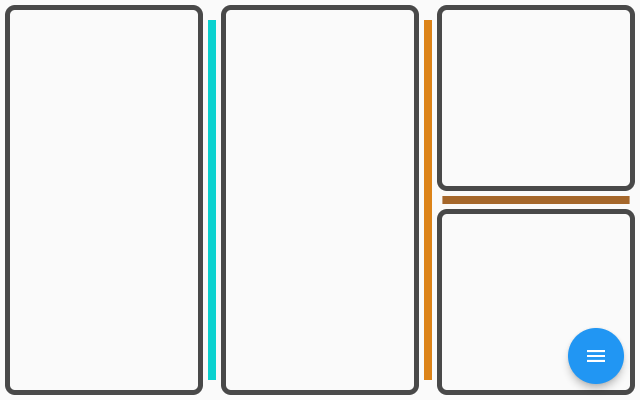
\includegraphics[width=0.5\textwidth]{Resizeline.png}
  \caption{Beschriebenes Beispiel mit der später beschreibenden Option \textit{resize} aktiviert}
\end{wrapfigure}
Es kann zum Beispiel, wenn es drei nebeneinander stehende Fenster gibt, das Linke in zwei geteilt werden, sodass es insgesamt vier Fenster gibt. Zwei sind links übereinander und die anderen Zwei sind rechts neben diesem Stapel horizontal angeordnet. 

Diese Variante wird bevorzugt, um mehr Möglichkeiten gegenüber eingeschränkten Rastern\footnote{Ein Raster beschränkt durch die Größe des Rasters sowohl die Größe und Position der Fenster, sowie deren Seitenverhältnisse (ein Fenster kann 1×1, 1×2, 2×2 usw. Kästen groß sein).} zu geben, wie sie zum Beispiel die \textit{Widgets} und \textit{Starticons} in Android nutzen.
Auf der anderen Seite wird eine Lösung mit Kollisionsabfrage verwendet, um den Prozess der Anordnung einfacher zu gestalten und Einschränkungen zu vermeiden, wie sie bei einem nicht vollständig angezeigten Widget auftreten können. 

%Wie oben bereits eingeleitet, wird dies mit einer Klasse namens Scaffolding realisiert. Diese hat intern eine Liste, die entweder Widgets oder ein Scaffolding speichern kann. Des Weiteren wird angegeben, ob die Elemente der Liste horizontal oder vertikal gespeichert werden. Im informatorischem Sinne ist dies ein Baum mit variabler Menge an Elementen und einer variablen Tiefe, bei der Scaffolding einem Knoten und ein Widget einem Blatt entspricht. 
Die Größe der Widgets kann vom Nutzer/von der Nutzerin variiert werden, indem die Änderung der Größe durch das Verschieben der Grenzen zwischen zwei benachbarten Widgets ermöglicht wurde. So sind Änderungen direkt sichtbar.
 Wird im Menü die Option \textit{resize} auswählt wird, erscheinen zwischen zwei Widgets (die im gleichen Scaffolding sind) farbige Linien, die sich bewegen lassen. Wenn diese bewegt werden, passen sich beide Widgets links und rechts automatisch an, sodass die Grenzen der beiden an der Linie liegen.
Für die Aktivierung dieser Option wurde eine Menüoption hinzugefügt, damit niemand aus Versehen etwas bewegt und damit das Anzeigen der Linien deaktivieren kann.\begin{wrapfigure}[15]{R}{0.25\textwidth}
  \centering 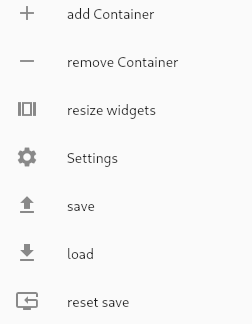
\includegraphics[width=0.25\textwidth]{Screenshot_20230113_192743.png}
  \caption{Drawer}
\end{wrapfigure}
Es gibt drei verschiedene Möglichkeiten mit dem Programm zu interagieren: den Drawer, das Popup-Menü und die separate Einstellungsseite. Diese existieren nur, wenn das Programm nicht auf dem E-Paper läuft.

\paragraph{Drawer}
Beim Drawer handelt es sich um eine Liste von Optionen, die sich durch das Herausziehen (engl. to draw) von links nach rechts (für Geräte mit einem Touchscreen) oder durch einen Knopf unten rechts öffnen lässt. Der Drawer bedeckt nicht den ganzen Bildschirm, sondern nur den linken Teil. Es lässt sich durch das Drücken neben den Drawer wieder schließen bzw. durch eine zum Öffnen entgegengesetzte Zieh-Bewegung. In ihr sind Optionen, wie das Speichern und Laden von Layouts, zu finden.
\paragraph{Popup-Menü} \label{popup}
Das \textit{Popup-Menü} ermöglicht die Konfiguration von Widgets. Es wird geöffnet, indem auf ein Widget doppelt geklickt wird und schließt sich wieder, wenn auf den Übernehmen- oder Abbrechen-Knopf gedrückt wird. Wenn das Widget nicht dem leeren Widget entspricht, wird eine Vorschau des Widgets links angezeigt und eine Liste aller Optionen rechts. Der Inhalt dieses Menüs umfasst sowohl einen für jedes Widget individuellen Teil als auch einige Widget-übergreifende Einstellungsmöglichkeiten. 
%perspektive, umstellung zu mehreren Seiten
Ein neues Widget kann erstellt werden, indem ein leeres Widget als Platzhalter eingefügt ist und in dessen Popup-Menü das Folge-Widget ausgewählt werden kann. 
%Das Erstellen neuer Widgets wurde dadurch gelöst, dass es ein leeres Widget gibt, in dessen Popup-Menü ausgewählt werden kann, wodurch dieses Widget ersetzt werden soll.
Es kann sowohl durch ein Scaffolding als auch durch ein Widget ersetzt werden. Wenn es durch ein Scaffolding ersetzt wird, kann auch ausgewählt werden, wie viele leere Widgets angezeigt werden sollen. 

\paragraph{Einstellungsseite}
Die Einstellungsseite bedeckt den ganzen Bildschirm und lässt sich über ein Feld im Drawer öffnen. Sie beinhaltet Einstellungen, die, im Gegensatz zum Drawer, nicht häufig geändert werden müssen, wie die IP-Adresse des Raspberry Pis.
\\\\
\begin{wrapfigure}[14]{l}{0.5\textwidth}
  \centering 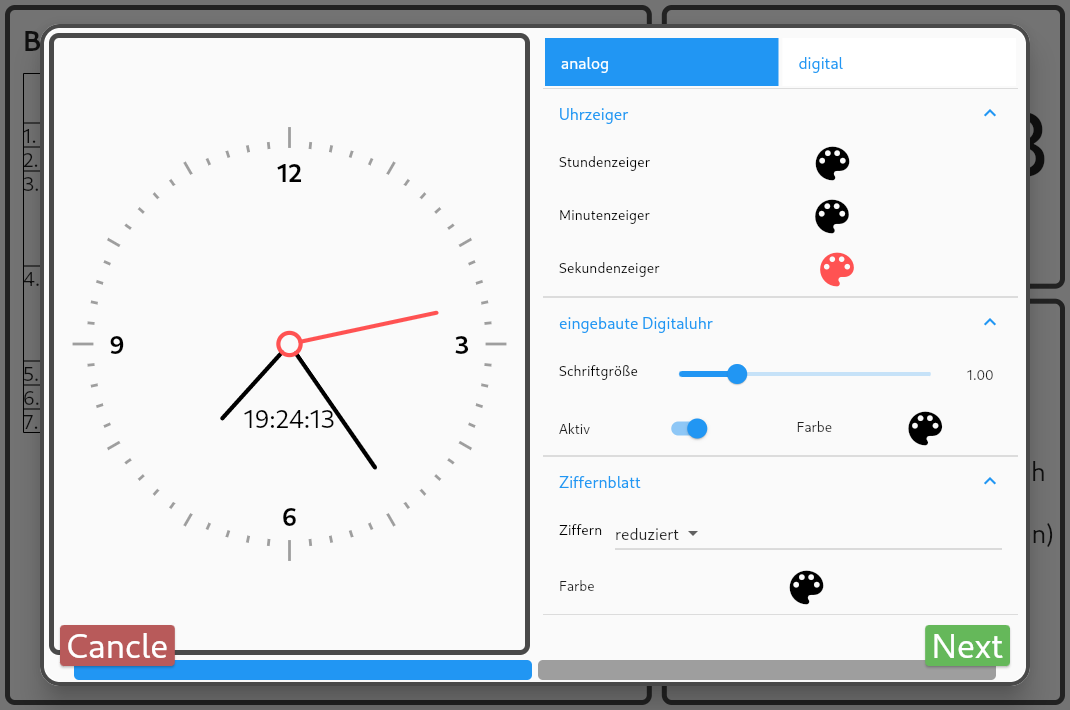
\includegraphics[width=0.5\textwidth]{Screenshot_20230113_192414.png}
  \caption{Popup-Menü der Uhr}
\end{wrapfigure}
\subsubsection{Datenspeicherung}
Für die Datenspeicherung werden, wie in Kapitel \ref{JSON} erwähnt, JSON Dateien verwendet. Es gibt zwei Dateien, über die die Informationen verteilt sind. Die erste (im Folgenden: allgemeine Konfiguration) speichert allgemeine Informationen, die Layout übergreifend benötigt werden. Ein Beispiel hierfür ist die IP-Adresse des Raspberry Pis. Die zweite Datei (im Folgenden: Layout-Konfiguration) speichert das Layout der einzelnen Widgets. Diese Dateien sind getrennt, damit  die Layout-Konfiguration unabhängig von der allgemeinen Konfiguration gewechselt werden kann. In der allgemeinen Konfiguration werden die Namen aller Layout Konfigurationen gespeichert, die sich wiederum in dem Ordner \textit{configs} befinden. Dadurch kann das Layout unabhängig von Werten wie der IP gespeichert oder geladen werden.

Im Detail wurde die Layout-Konfiguration so realisiert, dass es zwei verschiedene Klassen zur Konfiguration gibt, von denen jedes Widget je ein Objekt speichert. Die eine Konfiguration speichert Werte, die jedes Widget besitzt und die andere Informationen, welche spezifisch für einen Typ von Widget sind (wie die Farbe der Ziffern bei der Uhr). Beim Umwandeln in das Json-Format wird, neben diesen beiden Klassen, auch der Typ des Widgets gespeichert.

Scaffolding ist die einzige Ausnahme zu dieser Regel, da dieses ebenfalls andere Widgets speichert. Dies ist so realisiert, dass ein Scaffolding neben dem Feld \textit{gconfig} – für die allgemeine Konfiguration – ebenfalls mehrere Felder für die Speicherung der  – einzelnen Widgets hat. JSON benutzt sogenannte \textit{Key-Value pairs}. Dies heißt, dass jedem Wert ein eindeutiger Name zugewiesen ist. Dadurch sind klassische Listen nicht möglich, da bei diesen die Reihenfolge der Elemente zählt. Dies wird dadurch gelöst, dass den Widgets selbst ein variabler Name zugewiesen wird, der sich aus dem Wort \textit{Child} und einer Zahl, die abhängig von der Position des Widgets ist, zusammensetzt. Es kann ebenso Scaffoldings speichern, wie in Kapitel \ref{Container System} beschrieben wird.
%child ersetzen

\subsection{E-Paper}\label{Bildgenerierung}
Ausgehend von der Idee, etwas auf dem E-Paper-Display anzuzeigen, benötigt es einer Methode, ein Bild zu erstellen, das an den Controller des Displays gesendet werden kann. Eine hierbei notwendige Information ist, dass der Controller, der zum Ansteuern verwendet wird, kein HDMI Verbinder oder ähnliches (zum Beispiel VGA oder Display Port) besitzt, weswegen das Display standardmäßig nicht als Monitor erkannt wird. Bevor ein Bild zu einem Format umgewandelt werden kann, ist es notwendig, den Raspberry Pi zu täuschen, er sei an einen Monitor mit der Auflösung des E-Papers angeschlossen. 

Um den virtuellen Monitor zu erstellen, wird die X Erweiterung \textit{Resize and Rotate} (xrandr, engl. für Größe anpassen und rotieren) verwendet. Mit ihr lassen sich Monitorausgaben erstellen, selbst wenn kein Monitor angeschlossen ist. In diesem Fall müssen alle Informationen, die für die Kommunikation mit dem Monitor notwendig sind, angegeben werden. Da nur das Bild benötigt wird und nicht die Erstellung eines tatsächlichen HDMI Ausganges, sind die meisten Informationen unwichtig. Deshalb wird das Tool \textit{cvt} von Luc Verhaegen verwendet, um die gleichnamigen Informationen zu erstellen. 

\textit{Coordinated Video Timings} (cvt) ist ein Standard der Vesa\footnote{Vesa ist eine Organisation, die die meisten Standards für Monitore erstellt hat.} für \textit{Video Timings}. Video Timings umfassen eine Reihe von Informationen, die die Formatierung des Eingangsignals eines Monitors betreffen.

Sobald diese Monitorausgabe eingestellt ist, wird die grafische App gestartet. In festgelegten Intervallen (typischerweise eine Minute) wird das Bild der Monitorausgabe gelesen. Um das Bild an das E-Paper-Display senden zu können, muss es zuvor in ein schwarz-weißes Bild umgewandelt werden.

%Zusammengefasst wird erst ein Modus bei X hinzugefügt und als Output auf HDMI-1 verwendet. Anschließend muss jedes Mal, wenn das Bild erneuert wird, der Framebuffer von X11 ausgelesen werden und in ein Schwarz-Weiß Bild mit spezieller Formatierung umgewandelt werden.
\clearpage
\subsection{Gehäuse}
\begin{wrapfigure}[14]{L}{0.5\textwidth}
  \centering 
  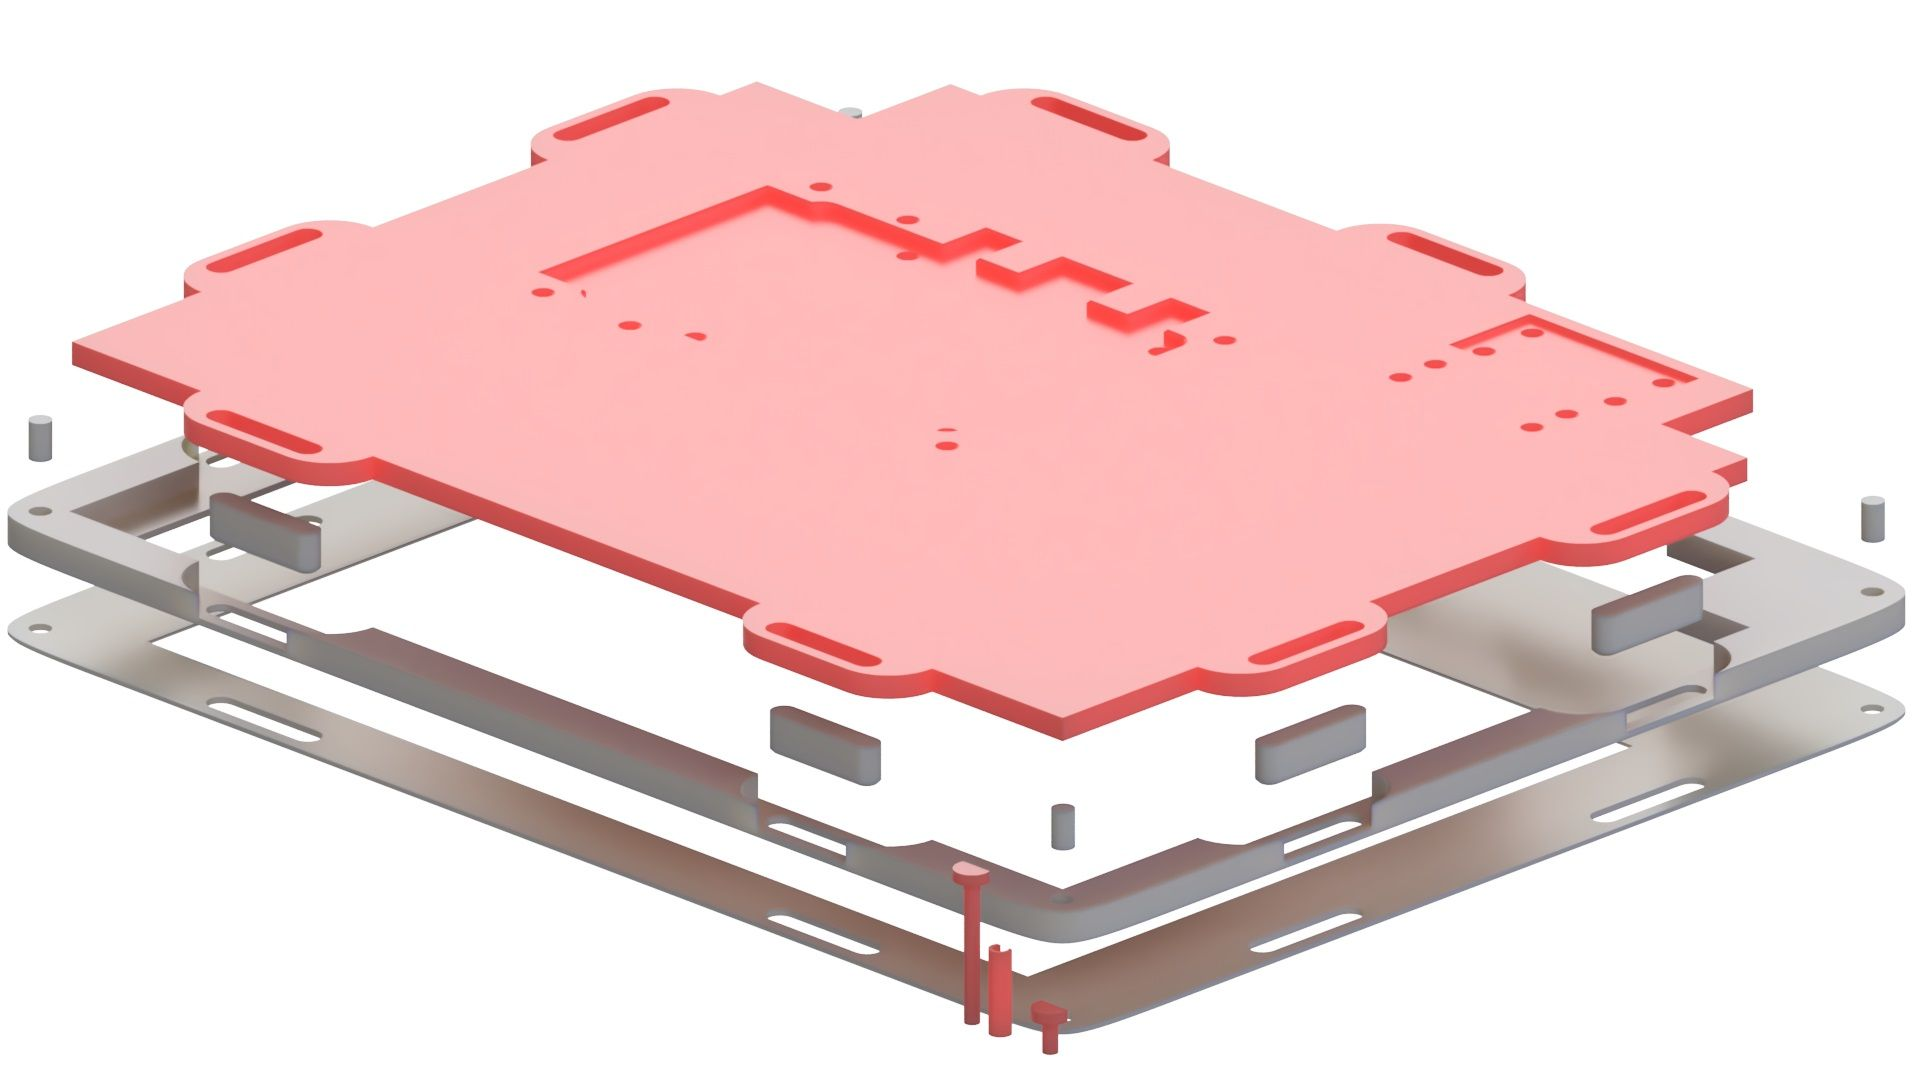
\includegraphics[width=0.5\textwidth]{gehaeuse.jpg}
  \caption{Orthografische Ansicht (selbsterstellt)}
  \label{gehaeuse}
\end{wrapfigure}
%zeichen einnfügen wie in Abbildung 2
%Gehäuse für mechanische Stabilität fpc und raspberry pi
Da der \textit{flexible printed circuit connector} (fpc connector, engl. für Verbinder für flexible gedruckte Platine) fragil ist, wurde ein Gehäuse konstruieren, an dem sowohl das Display als auch der Raspberry Pi montiert werden kann.  %https://www.raypcb.com/fpc-connector/

Es besteht aus drei Teilen, sowie einigen Pins und wird so montiert, dass erst das E-Paper in das Mittelstück gelegt wird und dann die Vorderseite daraufgelegt wird. Dabei ist darauf zu achten, dass das fpc auf der Seite mit der Aussparung liegt. Anschließend wird die Rückseite montiert. In die acht Aussparungen, die sich durch alle Ebenen ziehen, werden anschließend die großen Pins gesteckt. Zuletzt wird der Raspberry Pi mit den langen schmalen Pins befestigt und die Zusatzplatine ebenfalls auf die gleiche Weise mit den kurzen schmalen Pins montiert. Für diese sind extra Aussparungen vorgesehen (siehe Abbildung \ref{gehaeuse}, rotes Teil).

Für die Erstellung des 3D-Modells (siehe Abbildung \ref{gehaeuse})  wurde die CAD-Software \textit{Fusion 360} von \textit{autodesk} genutzt. Die Wahl dieser Software ist mit bestehender Erfahrung begründet.

%\begin{figure}[H]
%  \centerline{\includegraphics[width=0.6\textwidth]{Gehaeuse1.jpg}}
%  \caption{Orthografische Ansicht des Gehäuses. Die mittlere Aussparung in der roten Platte ist für den Raspberry Pi, während die oben rechts für die %Zusatzplatine ist. (selbsterstellt)}
%  \label{}
%\end{figure}

\section{Wissenschaftliche Erarbeitung}
\subsection{Analyse der Ausgangslage}
Bislang wurden einzelne Projekte mithilfe des E-Papers realisiert, unter anderem eine elektronische (Tür-) Beschilderung. Ferner haben drei Schüler der Ludwig-Geißler-Schule in Hanau ein digitales Türschild unter dem Namen „eSign“ entworfen. Ihre Arbeit beschränkt sich auf die Möglichkeit, eine beliebige Internetseite anzuzeigen und in einem Webinterface Türschilder zu verwalten \cite{eSign}. 
Weiterhin wurden elektronische Krankenhaus-Beschilderungen für ein effizienteres Krankenhausmanagement (Verbesserung der Krankenhaushygiene und die digitale Verwaltung von Zimmerbeschilderung und Raumbuchungssystem für Konferenzen) entwickelt \cite{Management_im_Krankenhaus}. 

\subsection{Strommessung}
Zur Beurteilung der anfallenden Kosten wurde der Stromverbrauch einer TV-Monitor-Anzeige mit der Technik des helper:Papers verglichen. Des Weiteren wurden die anfallenden Kosten mit aktuellen Strompreisen berechnet und eine Kosten-Nutzen-Analyse durchgeführt. 
\subsubsection{Stromverbrauch im Vergleich}
Von dem Kriterium des Stromverbrauchs ausgehend wurde der Verbrauch des E-Papers und des Raspberry Pis als auch der einer herkömmlichen Vertretungsplan-Anzeige (TV-Monitor) gemessen. Anzumerken ist, dass für die Vertretungsplan-Anzeige jede gängige Kombination aus Computer und Monitor eingesetzt werden kann. Die Verknüpfung des E-Paper-Displays mit einem Raspberry Pi verbraucht laut Eigenmessung 2,75 (± 0,05) Watt. Im Vergleich dazu verbraucht die Vertretungsplan-Anzeige (Monitor ohne Computer) selbst circa 169 Watt (Eigenmessung). Auf die Messung des Stromverbrauchs eines Computers wurde aufgrund der Aussagekraft der vorgenannten Werte verzichtet.  

Es wird angenommen, dass eine Vertretungsplan-Anzeige zehn Stunden am Tag (von sieben bis 17 Uhr), an fünf Schultagen pro Woche und 40 Wochen im Jahr (52 Wochen abzüglich 12 Ferien-Wochen) in Betrieb ist. Das ergibt eine Betriebsdauer von 200 Tagen pro Jahr
\newline

\noindent
\begin{tabular}{|l|c|c|c|} \hline
    Hardware & W * h = Wh & Wh * d = Wh pro Jahr & = kWh \\ \hline
   Monitor  & 169 * 10 = 1.690 & 1.690 * 200 = 338.000 & 338.000 / 1000 = 338\\ \hline
    E-Paper + RPI & 2,75 * 10 = 27,5 & 27,5 * 200 = 5.500 & 5.500 / 1. 000 = 5,5 \\ \hline
\end{tabular} 
\newline

\noindent
Legende: W = Watt; h = Stunde; d = Tage; kWh = Kilowatt pro Stunde
%\begin{tabular}{|l|c|c|c|} \hline
 %   Hardware & Watt*Laufzeit am Tag(in h) = Wh & Wh*Tage = Laufzeit pro Jahr(in Wh & = Kilowatt/Stunde (kWh) \\ \hline
  % Monitor  & 169 * 10 = 1.690 & 1.690 * 200 = 338.000 & 338.000 / 1000 = 338\\ \hline
  %  E-Paper+Raspberry Pi & 2,75 * 10 = 27,5 & 27,5 * 200 = 5.500 & 5.500 / 1. 000 = 5,5 \\ \hline
%\end{tabular}
\newline

\subsubsection{Stromkosten im Vergleich} \label{Stromkosten}
In der Rechnung wird ein günstiger Strompreis (Münster:ideal \cite{münsterideal}, gültig ab 1.02.2023) des lokalen Anbieters (Stadtwerke Münster) verwendet. Die Preise weichen je nach Tarif ab. Vergleichsweise wird ein treuerer Tarif (Mein Münster:strom \cite{mein_MünsterStrom}, gültig ab 14.10.2022) ebenfalls von den Stadtwerken Münster verwendet.   \newline
\noindent
\newline
\noindent
Strompreise (Brutto):
\newline
\begin{tabular}{|l|c|c|c|}
\hline
    Tarif &  Arbeitspreis in Cent/kWh & Arbeitspreis in Euro/kWh & Grundpreis Euro/Jahr\\ \hline
    Münster:ideal & 38,57 & 0,3857 & 122,37\\ \hline
    Mein Münster:strom & 66,90 & 0,6690 & 120,12 \\ \hline
\end{tabular}
\newline
\newline

\noindent
Strompreise auf das Beispiel angewendet:
\newline
\begin{tabular}{|l|c|c|}
\hline
      & E-Paper + Raspberry Pi & Monitor \\ \hline
    Münster:ideal  & 0,3857 * 5,5 = 2,1214 Euro & 0,3857 * 338 = 130,3666 Euro\\ \hline
    Mein Münster:strom  & 0,6690 * 5,5 = 3,6795 Euro & 0,6690 * 338 = 226,122 Euro \\ \hline
\end{tabular}
\newline

\noindent
% \textit{Mein Münster:Strom} \cite{mein_MünsterStrom} kostet vergleichsweise brutto 66,90 cent pro Kilowattstunde als Arbeitspreis mit einem Grundpreis von 10,01 Euro im Monat.
%\newline
%Preise für \textit{Mein Münster:strom} auf das Beispiel angewendet:
%\newline
%\begin{tabular}{|c|c|c|}
%\hline
 %    & Monitor & E-Paper + Raspberry Pi \\ \hline
  %  Preis gültig ab 14.10.2022 & 0,6690 * 338 = 226,122 Euro & 0,6690 * 5,5 = 3,6795 Euro \\ \hline
%\end{tabular}
%\newline
%
%\noindent
\paragraph{Beispiel einer Kosten-Nutzen-Analyse an einer fünfzügigen 
Schule mit vier Vertretungsplananzeigen: }

Die Beispielschule umfasst 25 Klassenräume der Unter- und Mittelstufe (Klasse fünf bis neun), 13 Kursräume der Oberstufe (Klasse zehn bis zwölf) sowie zwölf Fachräume (zum Beispiel für Informatik, Biologie, Chemie, Physik und Kunst).Die Ausstattung aller Räume mit einem helper:Paper umfasst somit 50 E-Papers und 50 Raspberry Pis. Um die Anschaffungskosten aus wirtschaftlichen Gründen gering zu halten, könnten in einem ersten Schritt die 25 Klassenräume der Unter- und Mittelstufe mit der neuen Technik ausgestattet und erprobt werden. Gerade die jüngeren Schüler können vom helper:Paper profitieren, da sie in der Schule keine Handys (Vertretungsplan-App) nutzen dürfen und dadurch auf die Vertretungsplan-Anzeige angewiesen sind. Durch die Einblendung einer möglichen Raumverlegung auf dem helper:Paper ist der Einsatz vor den Fachräumen zweitrangig, aber durch Anzeige von aktuellen Informationen (wie zum Bespiel „Achtung, hier wird eine Klausur geschrieben.“) nicht weniger sinnvoll.
\newline

\noindent
Stromkosten (mit \textit{Münster:ideal}) der Monitore im Vergleich zum E-Paper und Raspberry Pi: \newline
\begin{tabular}{lll}

    Vier Monitore:   & 130,3666 * 4 & = 521,4664 Euro (+ 122,37 Euro)\\
    50 E-Paper + 50 Raspberry Pis: & 2,1214 * 50 & = 106,0675 Euro (+ 122,37 Euro)\\  \hline
    \textbf{Ersparnis} & & \textbf{= 415,40 Euro} 
\end{tabular}
\newline

\noindent
\begin{tabular}{lll}
  Vier Monitore:   & 130,3666 * 4 & = 521,4664 Euro (+ 122,37 Euro) \\
    25 E-Paper + 25 Raspberry Pis: & 2,1214 * 25 & = 53,0338 Euro (+ 122,37 Euro)\\  \hline
    \textbf{Ersparnis} & & \textbf{= 468,43 Euro}
\end{tabular}
\newline

\noindent
Stromkosten (mit \textit{Mein Münster:strom}) der Monitore im Vergleich zum E-Paper und Raspberry Pi: \newline
\begin{tabular}{lll}
  Vier Monitore:   & 226,122 * 4 & = 904,488 Euro (+ 120,12 Euro)\\
    50 E-Paper + 50 Raspberry Pis: & 3,6795 * 50 & = 183,975 Euro (+ 120,12 Euro)\\  \hline
   \textbf{Ersparnis} & & \textbf{= 720,51 Euro}
\end{tabular}
\newline

\noindent
\begin{tabular}{lll}
  Vier Monitore:   & 226,122 * 4 & = 904,48 Euro (+ 120,12 Euro) \\
    25 E-Paper + 25 Raspberry Pis: & 3,6795 * 25 & = 91,9875 Euro (+ 120,12 Euro)\\  \hline
    \textbf{Ersparnis} & & \textbf{= 812,49 Euro}
\end{tabular}
\newline

\noindent
Ein günstiges E-Paper \cite{günstiges_E-Paper} und ein günstiger Raspberry Pi \cite{günstiger_RaspberryPi} kosten zusammen ungefähr 75,00 Euro.
\newline

\noindent
Preis für die Technik für 25 helper:Papers: 1.875,00 Euro
\newline
Preis für die Technik für 50 helper:Papers: 3.750,00 Euro

\paragraph{Rechenbeispiel bei der Anschaffung von 25 helper:Papers:} \mbox{}\vspace{2 ex}\\
%Für mehr E-Papers und Raspberry Pis erhöht sich die Zeit der Amortisierung.
Münster:ideal:
1.875 Euro / 468,43 = 4,0027 \rightarrow{Amortisierung nach vier Jahren}\\
Mein Münster:strom: 1.875 Euro / 812,49 = 2,3077 \rightarrow{Amortisierung nach zwei Jahren und vier Monaten}\mbox{}\vspace{2 ex}\\
Bei Mehranschaffung von E-Papers und Raspberry Pis erhöht sich die Zeit der Amortisierung entsprechend.

\section{Empirische Studie}

Nach der Kosten-Nutzen-Analyse wurde in Form einer Grundlagenstudie die potenzielle Verbesserung der Arbeitsqualität beziehungsweise des Zeitmanagements untersucht.

\subsection{Einleitung}
Raumänderungen, Vertretungs- und Freistunden werden in den Schulen über große Anzeigetafeln oder TV-Monitore an einem oder wenigen zentralen Ort angezeigt. Die Darstellung erfolgt vorwiegend in einer zeilenweisen Rotation, um alle Informationen darstellen zu können. 
Diese Informationen können auch über eine Vertretungsplan-App für Handys nachgeschaut werden; Handys dürfen im besten Fall nur von Oberstufenschüler*innen auf dem Schulgelände genutzt werden.

Das entwickelte helper:Paper soll vor Klassen-, Kurs- und Fachräumen zum Einsatz kommen und somit Raumnummernschilder und zentrale Anzeigentafeln oder TV-Monitore ersetzen. Angezeigt werden sollen sowohl individuelle Vertretungs- oder Belegungspläne als auch Informationen wie zum Beispiel die Uhrzeit, der Lehrername beim Elternsprechtag, Termine, Vertretungsaufgaben, Buspläne oder die aktuellen Corona-Vorschriften. Dies kann von jeder Schule individuell gehandhabt werden, da das helper:Paper mit einem Widget-Verfahren (siehe \ref{Widgets}) arbeitet, das per App angepasst werden kann.

In der empirischen Studie wurden Schüler*innen zur Problematik der zentralen Anzeige von Vertretungsplänen befragt und ob das helper:Paper für sie als Nutzer*in eine Lösung wäre (Optimierung der Arbeitsqualität).

Die zentrale Frage der Arbeit war, ob die Schüler*innen die Idee der Nutzung des helper:Papers als Vertretungsplan vor den Klassen-, Kurs- und Fachräumen als sinnvoll ansehen.

\subsection{Forschungsdesign und -methode} \label{Forschungsdesign und -methode}
Folgende Thesen werden in Bezug auf die Arbeitseffektivität durch den Einsatz des helper:Papers aufgestellt:
\begin{itemize}
    \setlength\itemsep{0em}
    \item verbessertes Zeitmanagement der Schüler*innen durch Weg- und Zeitersparnisse,
    \item keine Unterrichtsversäumnisse durch Zuspätkommen aufgrund von Raumsuche,
    \item weniger Störungen des Unterrichts,
    \item Erleichterung im Schulalltag, 
    \item die Schüler*innen sehen die Vorteile einer dezentralen Anzeige,
    \item die Schüler*innen stehen der neuen Technik positiv gegenüber (nicht geschlechts-spezifisch),
    \item Wunsch des Einsatzes des helper:Papers trotz technischer Unkenntnisse und
    \item das Alter der Befragten spiegelt sich in der Nutzung des helper:Papers wider. 
\end{itemize}
In der analogen und digitalen Umfrage werden systematisch Meinungen von Schüler*innen zum Thema Vertretungsplan, E-Paper und der Idee des helper:Papers gesammelt. 
Um präzise Daten vorzulegen und einen statistischen beziehungsweise numerischen Beweis für die Notwendigkeit des Projektes erbringen zu können, wird die quantitative Forschungsmethode angewendet \cite{Quantitative_Forschung}.
„In der quantitativen Forschung werden Ausschnitte aus der Realität gemessen, quantifiziert […] und statistisch ausgewertet“ \cite{Quantitative_Forschungsmethode_Definition}. Dadurch können neue Effekte entdeckt oder (Hypo-)Thesen überprüft werden.

\subsection{Datenerhebung}
Im Zuge der anonymen Umfrage wurden 211 Schüler*innen der Klassen fünf bis neun einer weiterführenden Schule im Münsterland befragt. Die Oberstufe befindet sich bei der zweizügigen Standort-Schule an einem anderen Standort.
Die Umfrage wurde mit \textit{Microsoft Forms}, eine für diesen Zweck von Microsoft entwickelte Software,  über einen Umfrage-Link, QR-Code und in gedruckter Form durchgeführt. In Forms können in einer „relativ einfachen, intuitiven Art und Weise“ \cite{Vorteile_Microsoft_Forms} Umfragen erstellt werden, an denen sowohl interne als auch externe Personen teilnehmen können. Zusätzlich zu der angebotenen Auswertungs- und Analysefunktion können Ergebnisse in Excel weiter analysiert werden. 
%Im Informatikunterricht wurde bereits mit Microsoft Excel gearbeitet, sodass grundlegende Kompetenzen vorliegen.

Die Umfrage-Rohdaten wurden mithilfe der Common Online Data Analysis Platform CODAP \cite{CODAP} ausgewertet und grafisch dargestellt. Microsoft Excel bietet eine Schnittstelle zwischen Microsoft Forms und CODAP. Mit den importieren Daten können uni-, aber auch bivariate Datenanalysen durchgeführt werden.

Die Umfrage wurde auf Grundlage der Internetseite „qualtrics.com“ strukturiert \cite{Erstellung_Fragebogen}.
Im Umfrage-Kopf wurde kurz beschrieben, „wer die Umfrage durchführt, welcher Zweck damit verfolgt wird und warum die [Schüler*innen] mitmachen [sollen]“ \cite[Struktur]{Erstellung_Fragebogen}.

Einleitend wurden demografische Daten wie Geschlecht und Unter-, Mittel- oder Oberstufe abgefragt.
Im Hauptteil wurden Alltagsproblematiken, die mit zentralen Anzeigetafeln oder TV-Geräten existieren (wie zum Beispiel Häufigkeit, vor dem falschen Klassen- beziehungsweise Fachraum zu stehen), erfragt. Um auch jüngere Schüler*innen befragen zu können, wurde auf eine einfache und gut verständliche Formulierung geachtet. Die Anrede „du“ sollte Nähe vermitteln. 
Die Fragen, ob die Schüler*innen schon etwas von einem E-Paper-Display gehört haben, bereitete sie auf die Folge-Fragen vor, da eine kurze Definition eingefügt wurde. 
Die anschließenden Fragen thematisierten die Idee und Nutzung des helper:Papers. Auch konnten im Schlussteil gewünschte Erweiterungsmöglichkeiten vorgeschlagen werden. Hier wurde auf ein Pflicht-Eingabefeld verzichtet.

\subsection{Datenauswertung}
Es konnten alle gesammelten Daten verwendet werden, da alle Pflichtfragen beantwortet wurden. Das ist möglich, da die Schüler*innen die Fragebögen unter Aufsicht von Lehrkräften ausgefüllt haben. 

\subsubsection{Univariate Datenanalyse} \label{Univariate Datenanalyse}

An der Umfrage haben insgesamt 211 Probanden/Probandinnen (im Folgenden: Probanden) teilgenommen, davon waren 98 (46 Prozent) weiblich und 113 (54 Prozent) männlich. Alle Probanden waren Schüler*innen einer weiterführenden Schule im Münsterland, von denen 67,77 Prozent (143 Schüler*innen) die fünfte bis siebte Klasse besuchen. Die restlichen 32,23 Prozent (68 Schüler*innen) besuchen die achte oder neunte Klasse. 

Noch nie vor einem falschen Klassen-, Kurs- oder Fachraum gewartet haben 55,93 Prozent (118 Schüler*innen) der Probanden und die restlichen selten, manchmal oder häufiger.
Es haben 84,36 Prozent (178 Schüler*innen) der Probanden angegeben, dass die Informationen des Vertretungsplans selten, manchmal oder oft überholt waren und sie es nicht schnell genug erfahren haben. 
Der Großteil der Probanden (101 Schüler*innen entspricht 48 Prozent) schaut ein Mal pro Tag auf die zentrale Anzeige des Vertretungsplans. Die durchschnittliche Häufigkeit beträgt 2,2 Mal täglich. 
Über dreiviertel der Probanden (163 Schüler*innen entspricht 77,25 Prozent) wünschen sich mehrere Bildschirme und Standorte für die Anzeige des Vertretungsplans. Auch findet die Mehrheit der Probanden (183 Schüler*innen entspricht 86,73 Prozent) es gut, wenn neben jedem Klassen-, Kurs- und Fachraum ein individueller Vertretungsplan hängen würde.

Unter einem Viertel der Probanden (48 Schüler*innen entspricht 22,75 Prozent) kannten bereits die Technologie eines E-Paper-Displays aus ihrem privaten Umfeld. Da kein hoher Bekanntheitsgrad des E-Papers erwartet wurde, wurde es kurz definiert.
Die Probanden bewerteten die Idee der Nutzung eines E-Papers als Vertretungsplan vor Klassen- und Fachräumen mit durchschnittlich 4,16 von fünf Daumen hoch.
Auch sehen über 80 Prozent (170 Schüler*innen entspricht 80,58 Prozent) der Probanden eine Erleichterung durch den Einsatz von E-Paper-Displays vor den Klassenräumen. 

Auf die Frage „Was könnte noch auf dem E-Paper-Display angezeigt werden?“, antworteten 128 Probanden (60,66 Prozent). Häufige Antworten waren: Countdown (Ferienanfang), Aktivitäten, ausstehende Aufgaben, Essenszeiten, vollständiger Lehrername auf dem Vertretungsplan (nicht nur das Kürzel) oder um wie viel Uhr der Unterricht beginnt.

\subsubsection{Bivariate Datenanalyse}
Aus Platzgründen wird in den folgenden Diagrammen Vertretungsplan mit "VP\grqq abgekürzt. \newline
Probanden der fünften bis siebten Klasse schauen durchschnittlich 1,93 Mal täglich auf die zentrale Vertretungsplananzeige, die restlichen 2,78 Mal (siehe Abbildung \ref{Häufigkeit Sicht auf den Vertretungsplan}).

Von 98 Probandinnen kannten 79 Prozent kein E-Paper-Display, von den 113 Probanden waren es 76 Prozent (siehe Abbildung \ref{Bekanntheit E-Paper}).
\begin{figure}[H]
  \centering
  \begin{minipage}[b]{0.49\textwidth}
    \includesvg[inkscapelatex=true,width=\textwidth]{Frage/3-6.svg}
  \caption{Ergebnis der empirischen Umfrage hinsichtlich der Häufigkeit der täglichen Sicht der Probanden auf den zentralen Vertretungsplan in Schulen unterteilt in Unter- und Mittelstufe}
  \label{Häufigkeit Sicht auf den Vertretungsplan}
  \end{minipage}
  \hfill
  \begin{minipage}[b]{0.49\textwidth}
    \includesvg[inkscapelatex=true,width=\textwidth]{Frage/1-9.svg}
  \caption{Ergebnis der empirischen Umfrage hinsichtlich der Bekanntheit eines E-Paper-Displays in Bezug auf das Geschlecht der Probanden\\}
  \label{Bekanntheit E-Paper}
  \end{minipage}
\end{figure}

Die Probanden (94 Prozent), die sich mehre Anzeigen für den Vertretungsplan wünschen, finden die Idee, neben jedem Fach-, Kurs- und Klassenraum einen individuellen Vertretungsplan zu hängen, gut (siehe Abbildung \ref{wunsch mehrere individuelle Anzeigen des vertretungsplans }).

Durch den Einsatz des helper:Papers neben Klassen-, Kurs- und Fachräumen sehen 163 Probanden (89 Prozent) eine Erleichterung im Alltag (siehe Abbildung \ref{Erleichterung durch helper:Paper}). 

\begin{figure}[H]
  \centering
  \begin{minipage}[b]{0.49\textwidth}
    \includesvg[inkscapelatex=true,width=\textwidth]{Frage/7-8.svg}
  \caption{Ergebnis der empirischen Studie hinsichtlich des Wunsches der Probanden nach mehreren Vertretungsplan-Anzeigen und der Frage, ob es eine gute Idee ist, neben jeden Raum einen individuellen Vertretungsplan zu haben}
  \label{wunsch mehrere individuelle Anzeigen des vertretungsplans }
  \end{minipage}
  \hfill
  \begin{minipage}[b]{0.49\textwidth}
    \includesvg[inkscapelatex=true,width=\textwidth]{Frage/8-11.svg}
  \caption{Ergebnis der empirischen Studie hinsichtlich der Erleichterung im Schulalltag und der Frage, ob es eine gute Idee ist, neben jeden Raum einen individuellen Vertretungsplan in Form eines helper:Papers zu haben.}
  \label{Erleichterung durch helper:Paper}
  \end{minipage}
\end{figure}
\clearpage
\begin{wrapfigure}[20]{l}{0.49\textwidth}
  \centering 
  \includesvg[inkscapelatex=true,width=0.49\textwidth]{Frage/9-10.svg}
  \caption{Ergebnis der empirischen Studie hinsichtlich des Aspektes Bekanntheit des E-Paper-Displays und der Bewertung der Nutzung eines E-Paper-Displays als Vertretungsplan vor den Räumen}
  \label{Sinnvoller Einsatz des helper:Papers}
\end{wrapfigure}
\mbox{}\\Da der geringe Bekanntheitsgrad eines E-Papers, wie schon im Kapitel \ref{Univariate Datenanalyse} beschrieben, zu erwarten war, wurde dieses in Frage 9 des Fragebogens (siehe \ref{Anhang}) kurz beschrieben. 

Probanden, die bereits vor der Umfrage ein E-Paper kannten, haben der Idee der Nutzung eines E-Paper-Displays als Vertretungsplan mit mehr als zwei von fünf Daumen hoch bewertet.
Die Mehrheit der restlichen Probanden haben den Einsatz mit fünf Daumen hoch angegeben (siehe Abbildung \ref{Sinnvoller Einsatz des helper:Papers}).
\\\\\\\\\\\\\\\\\\
\subsection{Auswertung und Bezug auf die Thesen} \label{Studie Auswertung}
Die unter Punkt \ref{Forschungsdesign und -methode} aufgestellten Thesen wurden unter Berücksichtigung der erhobenen numerischen Werte untersucht. Die empirische Studie soll grundsätzlich den Nutzen des helper:Papers untersuchen.

Über 44 Prozent der Probanden haben laut Umfragen schon mal vor einem falschen Klassen-,Kurs- oder Fachraum gewartet und kannten die Problematik, dass die Informationen des Vertretungsplans überholt waren und sie es nicht rechtzeitig erfahren haben (84,36 Prozent). Beides führte zur Verspätung einzelner Schüler*innen und zu verpasstem Unterrichtsstoff und -störungen. Somit können die Thesen, dass durch das helper:Paper das Zeitmanagement der Schüler*innen durch Weg- und Zeitersparnisse verbessert werden, verifiziert werden. Es gibt weniger Unterrichtsversäumnisse durch Zuspätkommen aufgrund von Raumsuche und damit weniger Störungen des Unterrichts. 

Über 80 Prozent der Probanden sahen in der Umfrage eine Erleichterung durch den Einsatz von individuellen Vertretungsplänen vor den Klassen-,Kurs- und Fachräumen. Folglich kann die These „Erleichterung im Schulalltag“ anhand der numerischen Datenanalyse bestätigt werden.
Auch kann die These, dass Schüler*innen Vorteile in einer dezentralen Anzeige des Vertretungsplans sehen, verifiziert werden: über 75 Prozent wünschten sich mehrere Bildschirme und Standorte für die Anzeige, durchschnittlich wurde der Idee der Nutzung eines E-Papers als Vertretungsplan-Anzeige vor den Klassen-, Kurs- und Fachräumen mit 4,16 von fünf Daumen hoch bewertet; der Median liegt bei 5. 
Anhand der bivariaten Datenanalyse kann die These, dass Schüler*innen gleichermaßen positiv gegenüber neuer Technik stehen, bestätigt werden. 

Von 98 Probandinnen kannten 79 Prozent kein E-Paper-Display und von 113 Probanden 76 Prozent. 
Trotz großer Unkenntnis in Bezug auf das E-Paper standen die Probanden der neuen Technologien (dem helper:Paper) laut Umfrage positiv entgegen und würden sich den Einsatz in ihrer Schule wünschen. Das Zitat einer Probandin „Wir brauchen das Ding!“ unterstreicht das Ergebnis.

Die These, dass das Alter der Befragten sich in der Nutzung einer dezentralen Anzeige widerspiegelt, kann mit der Stichprobe nicht verifiziert oder revidiert werden. Diese wurde mit der Annahme aufgestellt, dass auch Oberstufenschüler*innen befragt werden, die in der Schule die mobile Vertretungsplan-App nutzen dürfen. Dadurch wurde mit einem Unterschied in der Nutzung abhängig von Alter/Klassenstufe gerechnet. 

Ein eindeutiges Ergebnis der Umfrage ist, dass der Einsatz eines helper:Papers vor dem Klassen-, Kurs- und Fachraum als Vertretungsplan von der großen Mehrzahl (86,73 Prozent) aller Probanden begrüßt wird!


\section{Ergebnisse/Diskussion}
 In der abschließenden Diskussion zur Software, Hardware, Strommessung und der empirischen Studie werden Ergebnisse reflektiert, ein Fazit und Erweiterungsmöglichkeiten des helper:Papers sowie Potenziale für die Praxis aufgezeigt.


\subsection{E-Paper und Apps}
Die App erfüllt ihre Funktion und das E-Paper ist ansteuerbar. Da das Grundgerüst durch die Widgets modular aufgebaut ist, kann dieses in verschiedene Bereiche erweitert werden. Selbst das Backend, das auf dem E-Paper läuft, könnte auch für eine andere App verwendet werden. Dafür muss nur der Name der ausgeführten Datei geändert sowie der Webserver abgeschaltet werden. Die Anordnungsmöglichkeiten der App ermöglicht Flexibilität, während sie zugleich Struktur beim Konfigurieren geben. Des Weiteren lassen sich neue Widgets hinzufügen, ohne bestehenden Programmcode zu ändern.
%todo: auslagerung von 

\subsubsection{Auslagerung der Bildgenerierung auf dedizierten Computer}
Wie bereits in Kapitel \ref{wahl-hardware} erwähnt, muss die Bildgenerierung nicht zwingend auf dem Computer stattfinden, der für die Kommunikation mit dem E-Paper-Display zuständig ist. Bei einer Weiterentwicklung dieses Projektes wäre die Trennung dieser beiden Aufgaben eine Möglichkeit den Stromverbrauch zu senken, da auf einem Computer für mehrere E-Papers die grafische App laufen kann. Hierbei wäre die einfachere Lösung, auf dem Computer mehrere grafische Apps laufen zu lassen. Dies könnte einen hohen Speicherverbrauch, sowohl auf der CPU, als auch auf der GPU, verursachen. Um dies zu minimieren, könnte die grafische App mit dem Feature erweitert werden, für mehrere E-Papers das Bild generieren. Das könnte so gelöst werden, dass die grafische App das Bild ändert. So könnte bei einer Wiederholrate von einem Bild pro Minute, wenn das Erstellen eines Bildes eine Sekunde braucht, eine App 60 helper:Papers mit einem Bild versorgen.

\subsubsection{Weitere Verbesserungsmöglichkeiten und technische Herausforderungen}
Bei der App wäre eine mögliche Änderung bezüglich der Nutzbarkeit das Hinzufügen weiterer Widgets. Mit den momentanen Widgets ist es möglich, die Idee zu erfassen und auch in der Schule einzusetzen, für die Schule wäre jedoch ein extra Fenster mit Informationen über die aktuellen Klausuren hilfreich. Es wird meist nur der Termin einer Klausur im Voraus mitgeteilt und nicht der Raum. Dieser ist nur durch den Vertretungsplan ablesbar. Auch fehlt bei dem Belegungsplan die Möglichkeit, Raumänderungen zu anderen Räumen zu anzeigen. Angenommen, ein Raum wird für die Oberstufe geändert. In diesem Fall wird nur vor dem Raum, zu dem geändert wurde, die Änderung angezeigt. Vor dem ursprünglichen Raum ist diese Information nicht ablesbar.
Da VpMobil nicht speichert, welcher Raum der Normalfall ist, wäre die Verwendung einer anderen Schnittstelle außerhalb von VpMobil vorteilhaft.

\subsection{Beurteilung Strommessung}\label{Strommessung}
Grundsätzlich gilt, je teurer der Strom ist, desto schneller sind die Kosten der Technik durch die Stromersparnisse abgedeckt. 

Aktuell sind die Kosten der Technik nach ungefähr zwei beziehungsweise vier Jahren für 25 helper:Papers amortisiert (Auf Grundlage der aktuellen Strompreise der Stadtwerke Münster \ref{Stromkosten}).
Bei diesem Vergleich wurden die Anschaffungskosten neuer TV-Monitore nicht mit eingerechnet.  

Außerdem geht der Stromverbrauch des E-Papers fast ausschließlich von dem Raspberry Pi aus. Das E-Paper selbst verbraucht, wenn es nicht aktualisiert wird, nur 0.3 Watt \cite{ourepd}.
Dies könnte noch weiter gesenkt werden, wenn der Controller nach jedem Neuladen abgeschaltet werden würde. Dies ist in dieser Nutzung möglich, da das Konfigurieren mit unter einer Sekunde weniger Zeit in Anspruch nimmt, als das Aktualisierungsintervall. 

Auch könnte bei Verzicht auf eine Uhr das Intervall so weit gesenkt werden, dass der Raspberry Pi zwischen Intervallen abgeschaltet wird. Dies benötigt jedoch externe Hardware, die für das Wiederanschalten des Raspberry Pis sorgt, da dieser weder \textit{Wake on LAN} - eine Möglichkeit, einen Computer über LAN wieder anzuschalten -, noch einen Stromsparmodus (\textit{hibernate}) besitzt. Da sowohl der Monitor als auch das helper:Paper eine externe Hardware zum Stromsparen/Aus- und Anschalten benötigt, wurde das nicht in der Kosten-Nutzen-Analyse berücksichtigt. 

\subsection{Beurteilung Empirische Studie}
Die Umfrage wurde von den 211 Schülern*innen gut angenommen; zum Projekt selbst gab es keine Verständnisfragen. Lediglich die jüngeren Schüler*innen kannten den Begriff „divers“ nicht. Da die Umfrage von ihren Lehrer*innen betreut wurden, die das Projekt gerne unterstützt haben, konnte der Begriff schnell erklärt werden. Die Auswahlmöglichkeit „divers“ beim Item „Geschlecht“ wurde gegeben, um niemanden aus der Umfrage auszuschließen.

Anhand der Probanden wurde die Notwendigkeit und Nützlichkeit des helper:Papers bestätigt, sodass aufgrund dieses eindeutigen Ergebnisses auf einen Hypothesentest verzichtet wurde.

Die empirische Studie ergab, dass eine nahe Entwicklung mit möglichen Nutzern*innen hilfreich sein kann. Aufgrund der unterschiedlichen Sichtweisen der Nutzer*innen auf das Projekt konnten diese neue Impulse und Anregungen geben.

Die Umfrage könnte noch auf Lehrkräfte und Verwaltungs- und Fachangestellte ausgeweitet werden, wobei bereits involvierte Lehrkräfte mündlich ein durchweg positives Feedback gegeben haben. Auch ohne Befragung dieser Gruppen ist offensichtlich, dass durch den Einsatz des helper:Papers Ressourcen, Arbeitsmittel wie zum Beispiel Papier und auch Arbeitszeit durch den Wegfall der manuellen Beschriftung der Räume, eingespart werden.

Wie anfangs erwähnt, sind weitere mögliche Anwendungsorte Unternehmen, öffentliche Gebäude oder der häusliche Gebrauch, zu denen jeweils noch weitere Umfragen gestartet werden könnten.

\subsection{Zusammenfassung}
Die Anschaffung des helper:Papers wird sowohl die Digitalität der Schulen fördern als auch auf Dauer eine ressourcenschonende Alternative zu den Vertretungsplan-Anzeigen und den Papier-Aushängen darstellen. Mit dem Stromverbrauch eines herkömmlichen Monitors können zahlreiche helper:Paper betrieben werden. Somit ist die Antwort auf die Frage, ob das helper:Paper dazu beitragen kann, den Stromverbrauch zu senken: Ja, ein helper:Paper kann helfen, Ressourcen einzusparen, wobei die Einsparung von Anzahl der neu anzuschaffenden Geräten und der Anzahl der zu ersetzenden Geräte abhängig ist. 

Um die Kosten der neuen Hardware (E-Paper und Raspberry Pi) gering zu halten, kann die Installation der helper:Paper in einem ersten Schritt vor den Klassenräumen (der Unter- und Mittelstufe) und später vor jedem Raum erfolgen. Trotz der entstehenden Kosten ist das Projekt helper:Paper, zum Beispiel durch Investitionen des Staates in technische Infrastruktur der Schule oder durch die Amortisierung, finanzierbar. Die Anschaffungskosten können dabei überschaubar sein. Einfache Geräte werden bereits für circa 50,00 Euro \cite{günstiges_E-Paper} angeboten. Ein Raspberry Pi ist für ungefähr 25,00 Euro \cite{günstiger_RaspberryPi} zu kaufen. Komfortablere Geräte, wie das in unserer Arbeit verwendete, kosten circa 170,00 Euro \cite{ourepd}.

Der Einsatz des helper:Papers hat positive Auswirkungen auf die Arbeitseffektivität. Insbesondere das Zeitmanagement der Schüler*innen und auch der Lehrkräfte sowie der Verwaltungs- und Fachkräfte verbessert sich, da Arbeitsschritte eingespart werden. Somit wird diese Frage (siehe \ref{Verbesserung Arbeitsqualität?}) positiv beantwortet.

Aus diesen Gründen erweist sich die Anschaffung des helper:Papers als sinnvoll und außerordentlich hilfreich!
\section{Programmcode und Umfrage} 
\label{Anhang}
\begin{wrapfigure}[14]{l}{0.3\textwidth}
  \centering 
  
\includegraphics[width=0.3\textwidth]{qr.png}
  \caption{Link zum Github repository}
\end{wrapfigure}
Den Programmcode der grafischen Applikation und des E-Papers, sowie die Umfrage und Umfrageergebnisse können auf \textit{Github} unter \href{https://github.com/Projektkurs/6dETv7SCVQ26Dfri}{https://github.com/Projektkurs/6dETv7SCVQ26Dfri} abgerufen werden. Dort ist ebenfalls der Latex Code zu finden, welcher zur Erstellung dieses PDFs, mit der Software \textit{Overleaf}, genutzt wurde. Der Name des Repositorys wurde Zufalls-generiert, damit das Projekt nicht schon vor der Präsentation im Internet gefunden werden kann.%new lines needed for printbibliography, vspace doen't work
%\addcontentsline{toc}{section}{References}
%\printbibliography
\section{Danksagung}
Abschließend möchten wir uns bei allen bedanken, die uns bei der Umsetzung unseres Projektes unterstützt haben.
Unser besonderer Dank gebührt unserem Betreuer Herrn Hendrik Büdding, der unser Projekt von der ersten Idee über die Alphaversion bis hin zum jetzigen Produkt begleitet hat.

Auch möchten wir uns bei unseren Mitschüler*innen des Projektkurses bedanken. Ihre Impulse und Kritiken haben uns vorangebracht. Durch diesen Austausch ist aus unserer Idee erst das helper:Paper geworden.

Ein weiterer Dank geht an die Anne-Frank-Gesamtschule Havixbeck-Billerbeck, insbesondere an die Abteilungsleiterin Frau Thomas, die die Durchführung der Umfrage am zweizügigen Teilstandort in Billerbeck möglich gemacht hat. Deren Schüler*innen haben an unserer Umfrage zur Nutzung des helper:Papers teilgenommen und durch ihre Teilnahme an der Befragung bestätigt, dass unser Projekt zukunftsträchtig ist – vielen Dank!

\newpage
\section{Literatur}
\begingroup
\renewcommand{\section}[2]{}
\printbibliography
%\printbibliography[heading=bibintoc]
\endgroup
\newpage\section*{\bfseries Selbstständigkeitserklärung}
\vspace{3ex}
Hiermit bestätige ich, dass ich das Projekt, welches die Projektarbeit, die Umfrage, das Gehäuse und das Programm umfasst, selbstständig erstellt habe und nur die angegebenen Hilfsmittel verwendet habe.\\

\includegraphics[width=0.65\textwidth]{selbstständigkeitserklärung/BMK-Selbstjpg.jpg}\mbox{}\\\\

\includegraphics[width=0.65\textwidth]{selbstständigkeitserklärung/Linda-Selbst.jpg}
%\vspace{10ex}
%\newline
%\vspace{1ex}
%\clearpage \vspace{10ex}
%Münster, den \today \qquad .............................................................................. 
%\newline \noindent \hspace*{15.5em} Linda Gemeinhardt 
%\noindent
%\newline
%\newline
%\newline
%\newline
%\clearpage \vspace{10ex}
%Münster, den \today \qquad ..............................................................................
%\newline \noindent \hspace*{15.5em} Ben Mattes Krusekamp
\end{document}